\section{Experimental Results}\label{sec:exp}
\graphicspath{{../../plots/}}
\epstopdfsetup{outdir=./figures/}

In this section we evaluate empirically the optimizations outlined in \cref{sec:yourmethod}. Every code version is tested for correctness on a small size example with hand-computed output and on several large-size random instances with output given by the naive implementation.

\mypar{Experimental setup}
For the empirical evaluation of the code, we use a Skylake processor (3.5 GHz, L1 cache 128 KB, L2 cache 1 MB, L3 cache 6 Mb). The compiler used is g++ with flags "-O3 -fno-tree-vectorize -march=native -mavx". The matrix size varies in the range $[30,1000]$.

\mypar{Results: operational count optimization}
We first evaluate the gain the in runtime due to the optimization in the operational count performed with the trick as in \cref{equation:qmmm_smart}. From \cref{figure:performance_qmm_kernel} we can see the decrease in performance of the trick version with respect to the naive implementation. \Cref{figure:cycles_qmm_comparison} shows that the operation count optimization gives an overall speed-up of $15 \%$ (this is the difference in run time between \emph{naive} and \emph{naive\_trick}). In \cref{figure:Cycles_trick} we can see the contribution of each function of the vanilla implementation of the pipeline to the overall runtime. In the following the trick version is further optimized.

\begin{figure}[h]
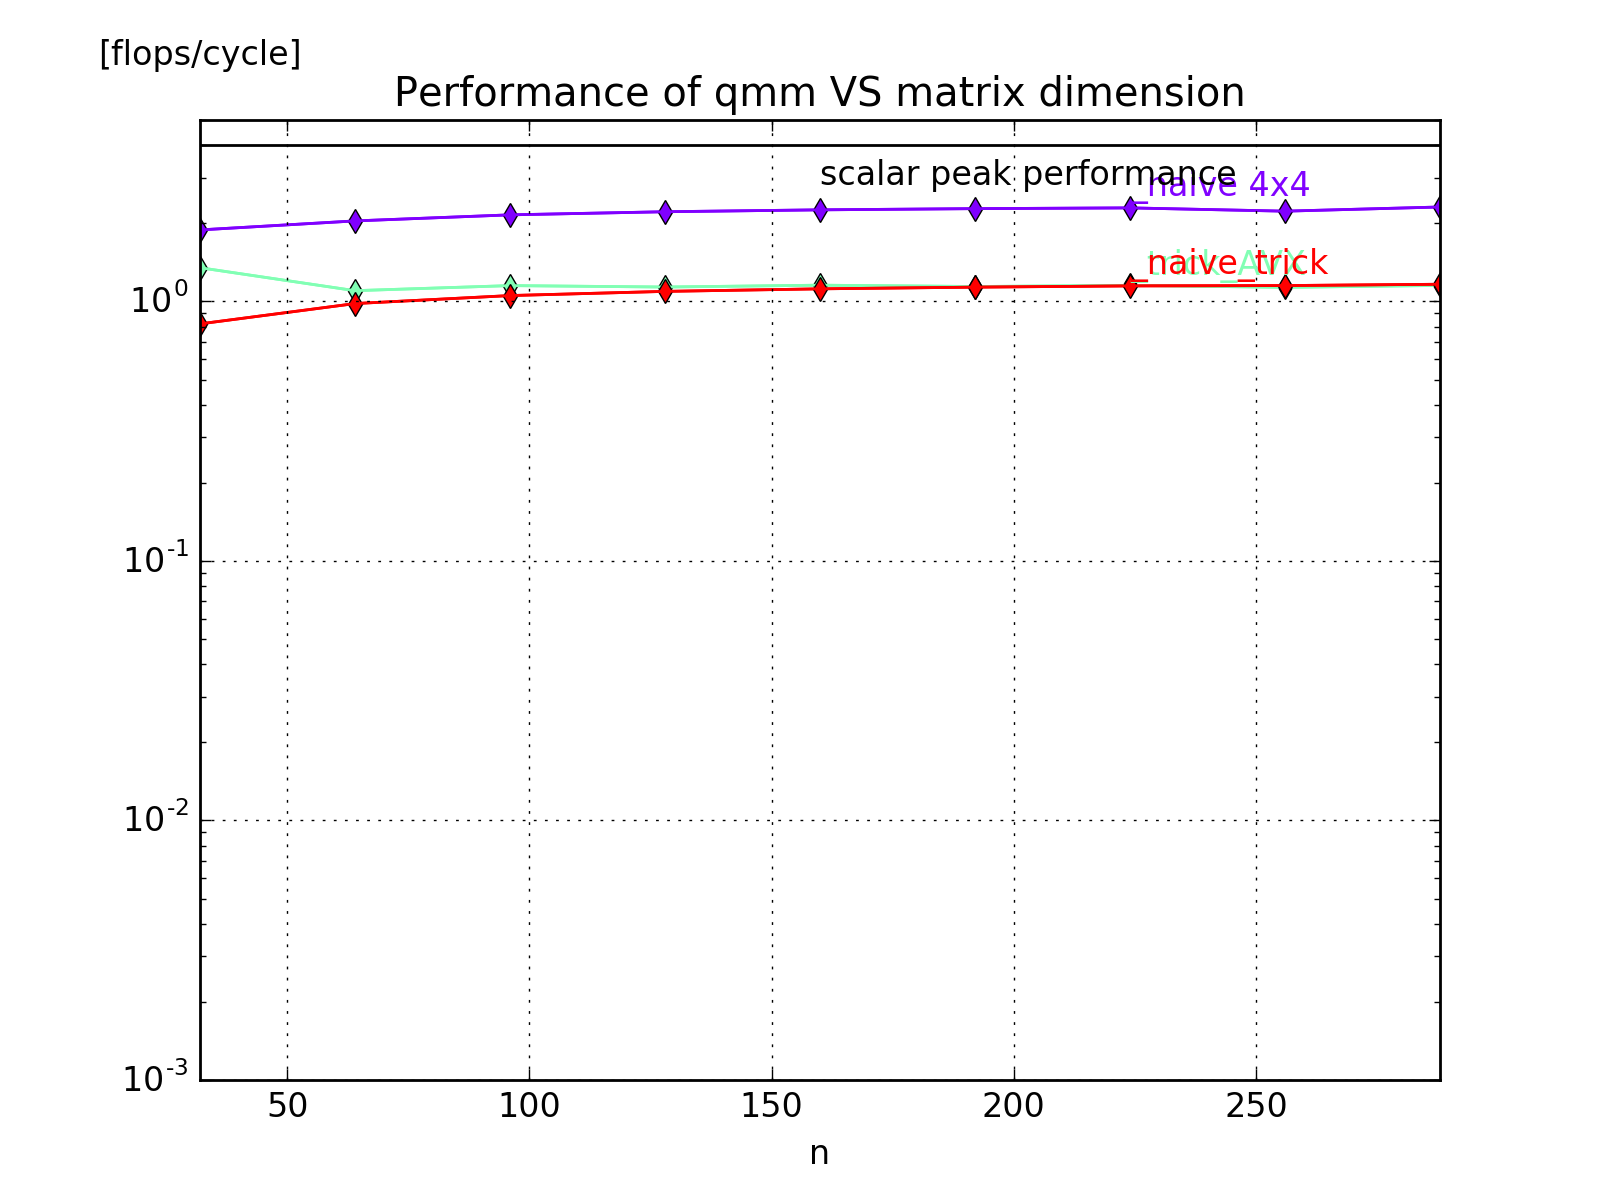
\includegraphics[width=0.5\textwidth]{Performance_qmm.eps}
\caption{Performance plot for the QMM kernel}
\label{figure:performance_qmm_kernel}
\end{figure}

\begin{figure}[h]
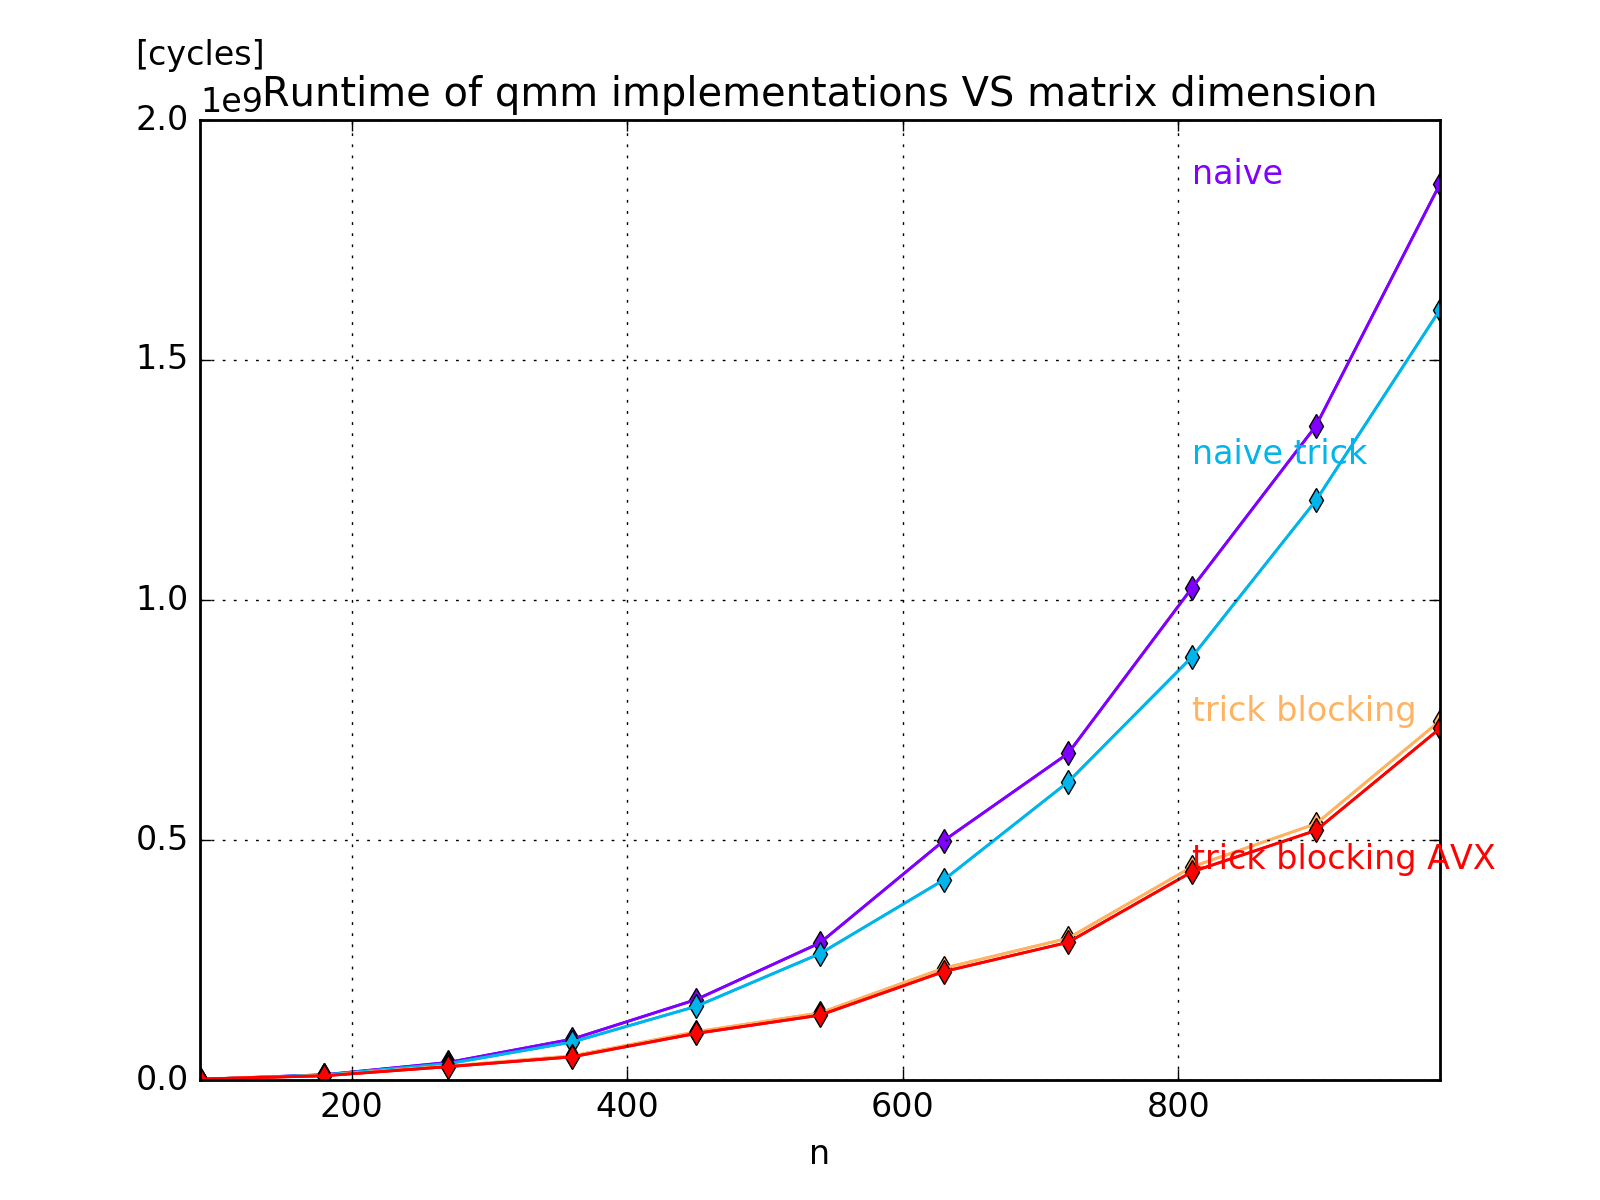
\includegraphics[width=0.5\textwidth]{Cycles_qmm_comparison.eps}
\caption{Runtime plot of the overall pipeline}
\label{figure:cycles_qmm_comparison}
\end{figure}

\begin{figure}[h]
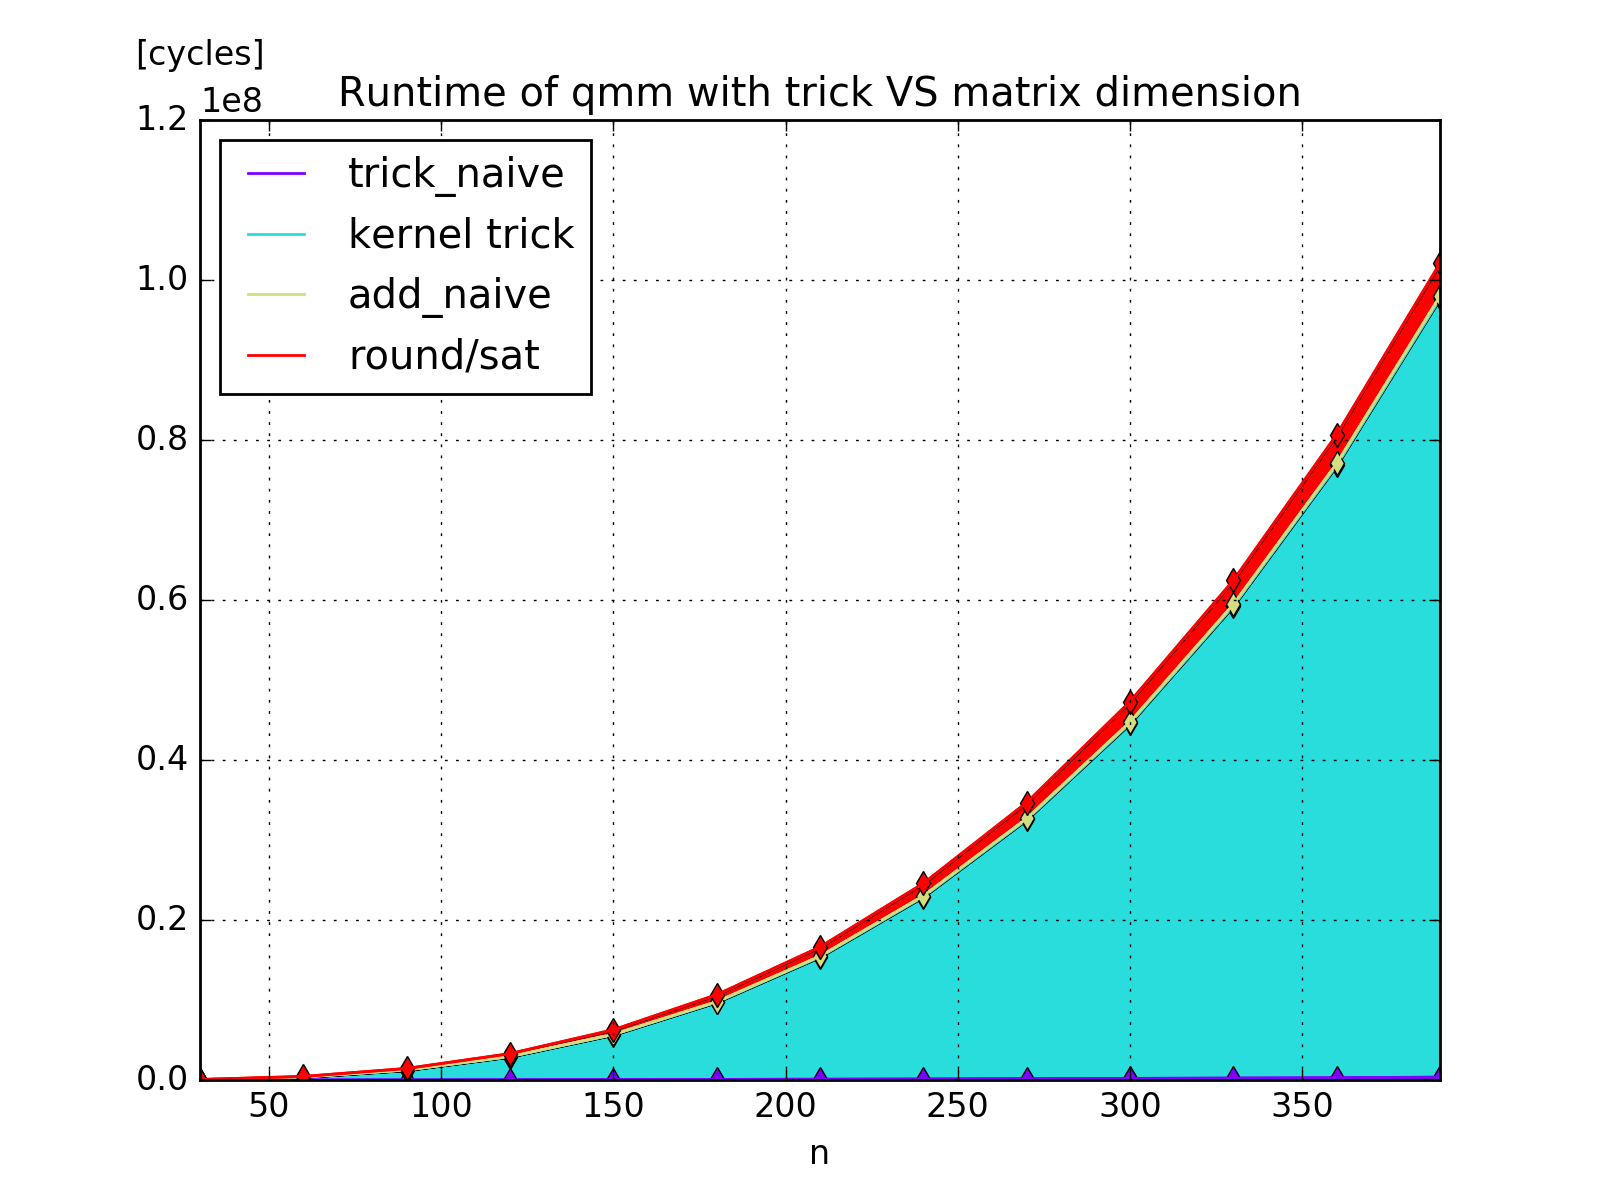
\includegraphics[width=0.5\textwidth]{Cycles_trick.eps}
\caption{Contribution of each naive-version sub-function in the overall runtime.} 
\label{figure:Cycles_trick}
\end{figure}


\mypar{Results: blocking for MMM}
The blocking parameter used is $N_b = 30$ for cache blocking  and $n_b = 3$ for register blocking, as described in \cref{sec:yourmethod}. \Cref{figure:performance_qmm_kernel} shows the gain in performance with respect to the \emph{naive\_trick} implementation. The performance gain for large  large $n$ is approximately $2$X. Note that the blocking parameter for cache and for register are not fine tuned, so a further speed-up could be possible.


\mypar{Results: vectorization} 
In this paragraph we evaluate the performance gain thanks to vectorization for \emph{trick\_vector}, \emph{quantize}, \emph{add\_trick\_vector} and \emph{round\_saturation} as outlined in \cref{sec:yourmethod}. \Cref{figure:performance_add_vector} and \cref{figure:performance_trick_vector} show a linear increase of the performance for small instances. This is due to a border effect. The instance size in the  performance plot are not in general a multiple of the vector size ($16$X$16 \ Bits$), hence for small instance size the scalar computation is be non-negligible. Moreover the scalar contribution decreases linearly with $n$.

\begin{figure}[h]
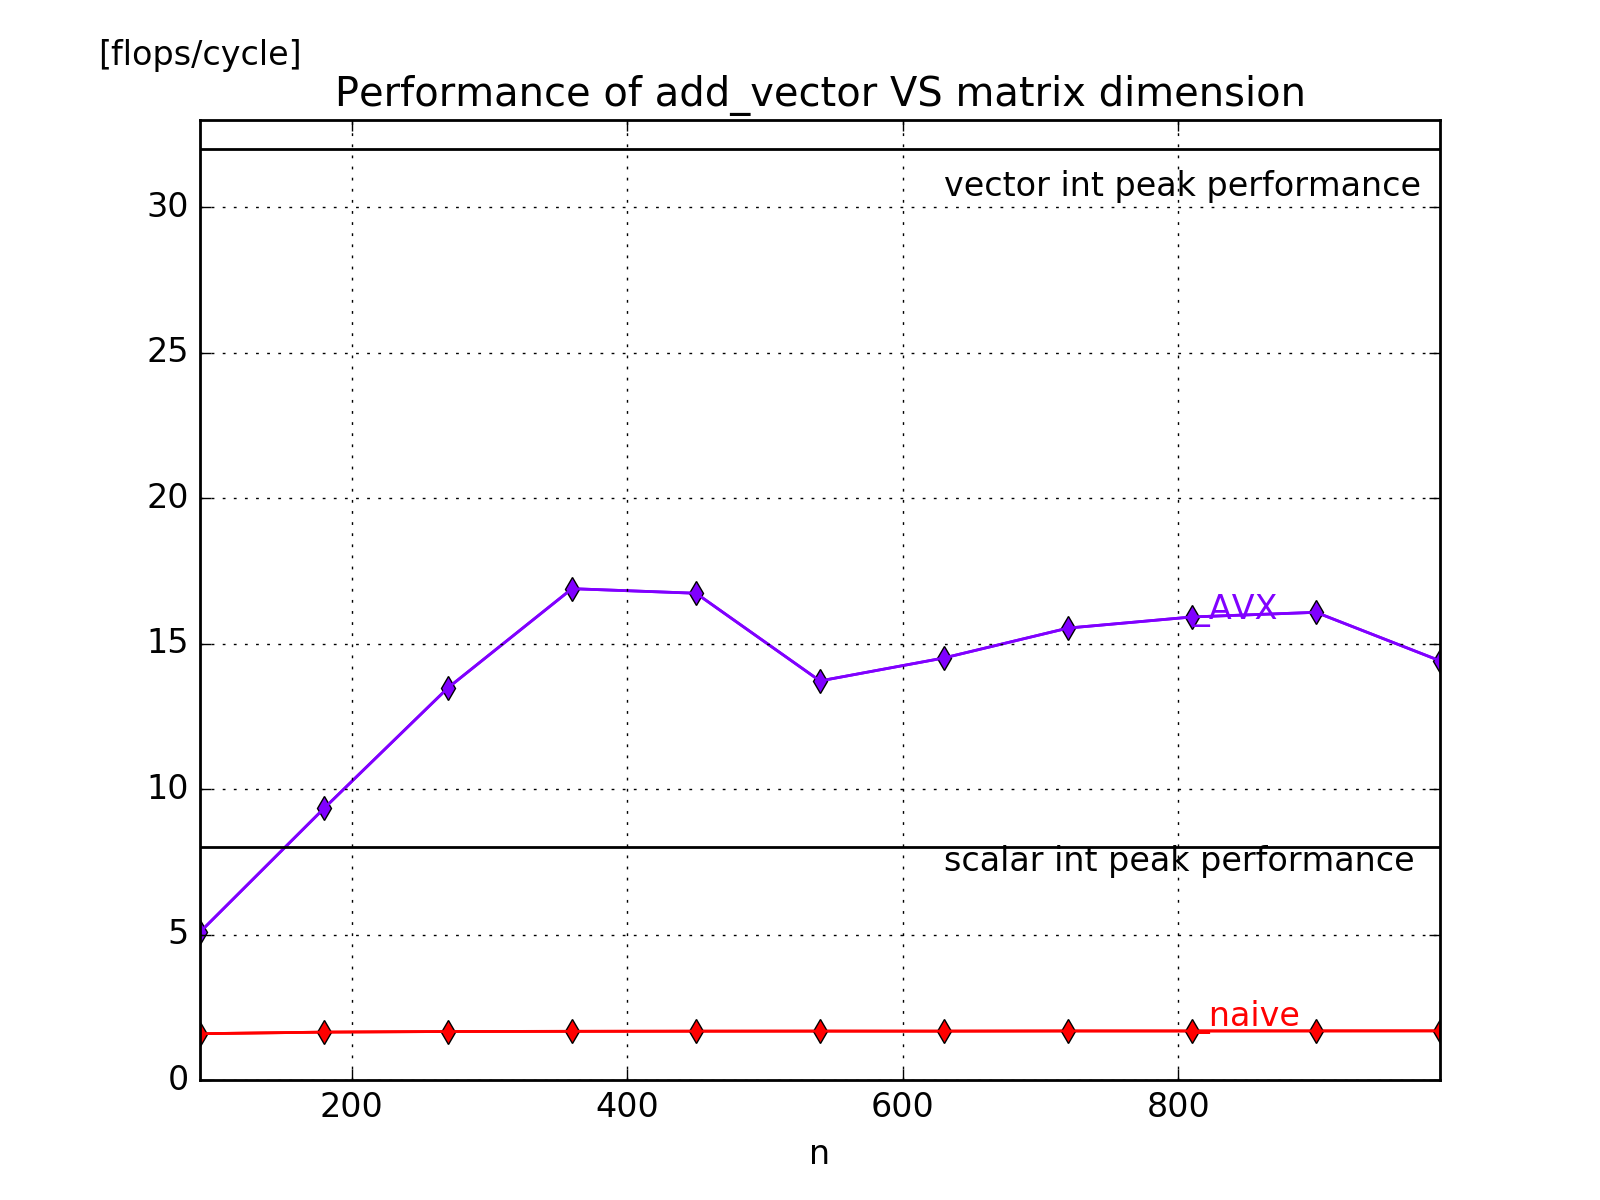
\includegraphics[width=0.5\textwidth]{Performance_add_vector.eps}
\caption{Performance plot of the function \emph{add\_vector}}
\label{figure:performance_add_vector}
\end{figure}

\begin{figure}[h]
	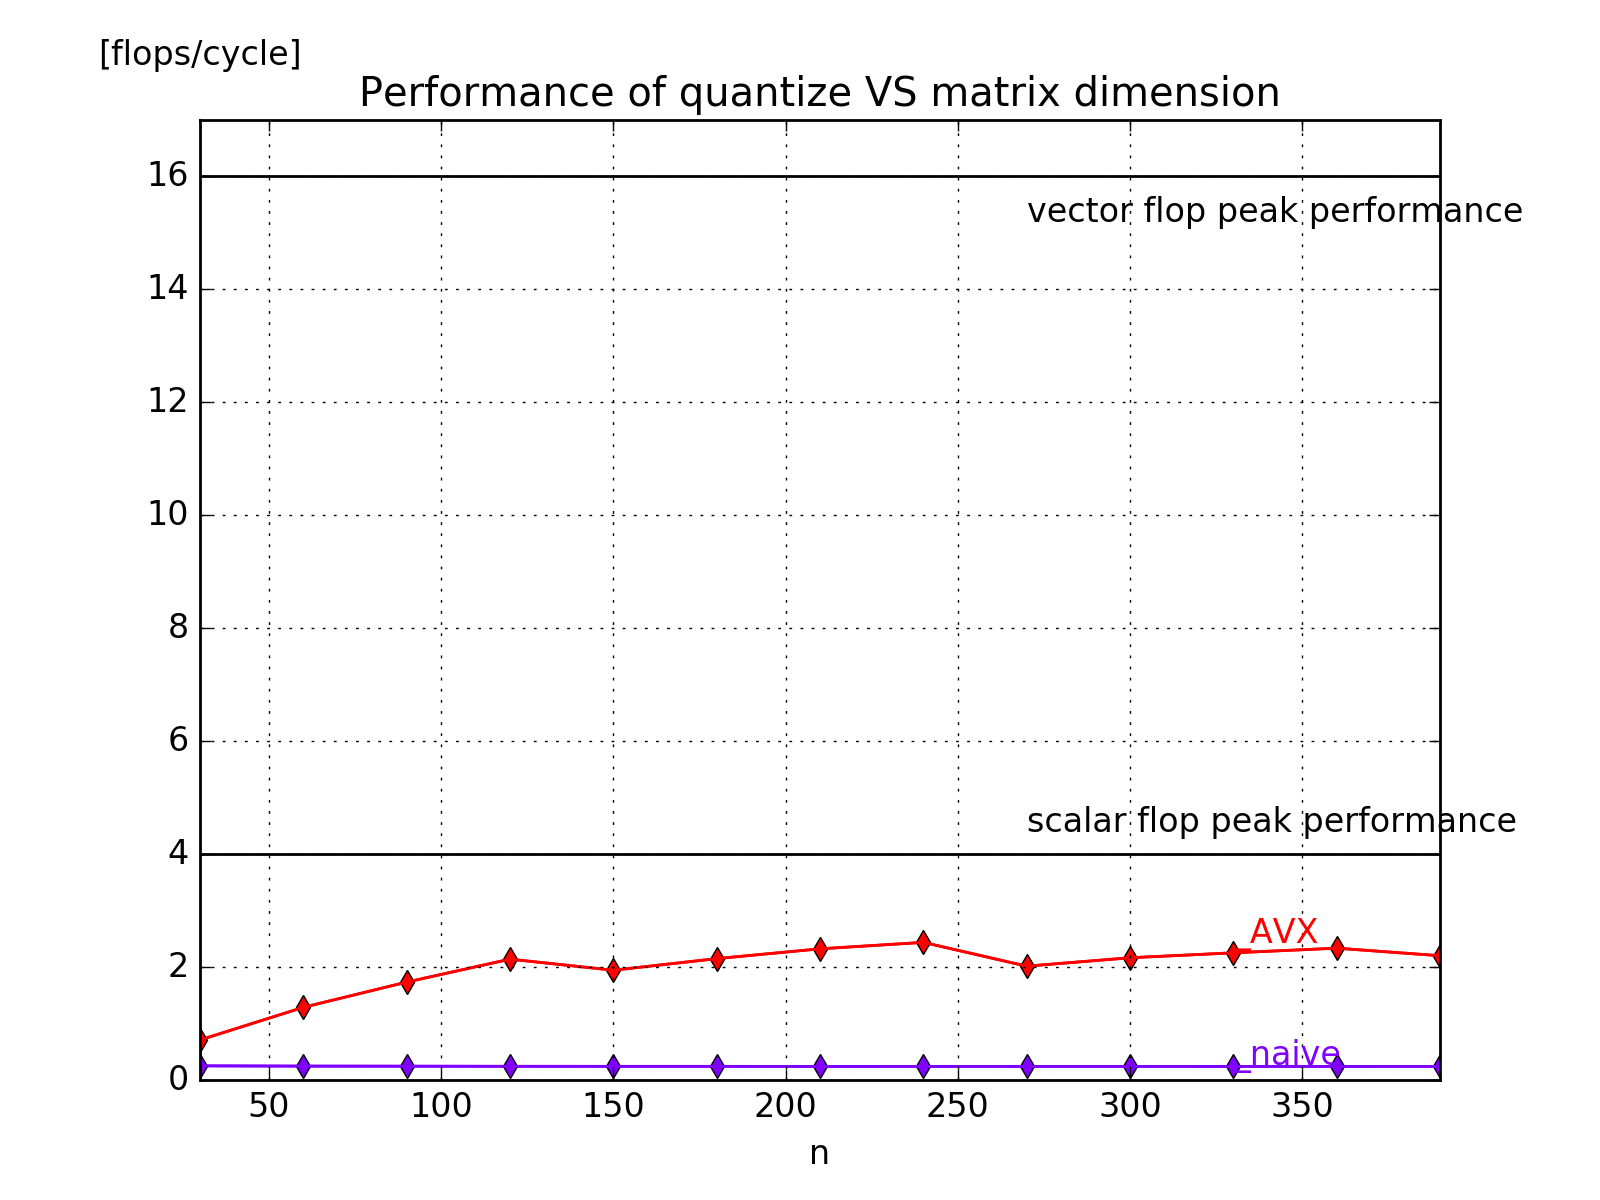
\includegraphics[width=0.5\textwidth]{Performance_quantize.eps}
	\caption{Performance plot of the function \emph{quantize}}
	\label{figure:performance_quantize}
\end{figure}

\begin{figure}[h]
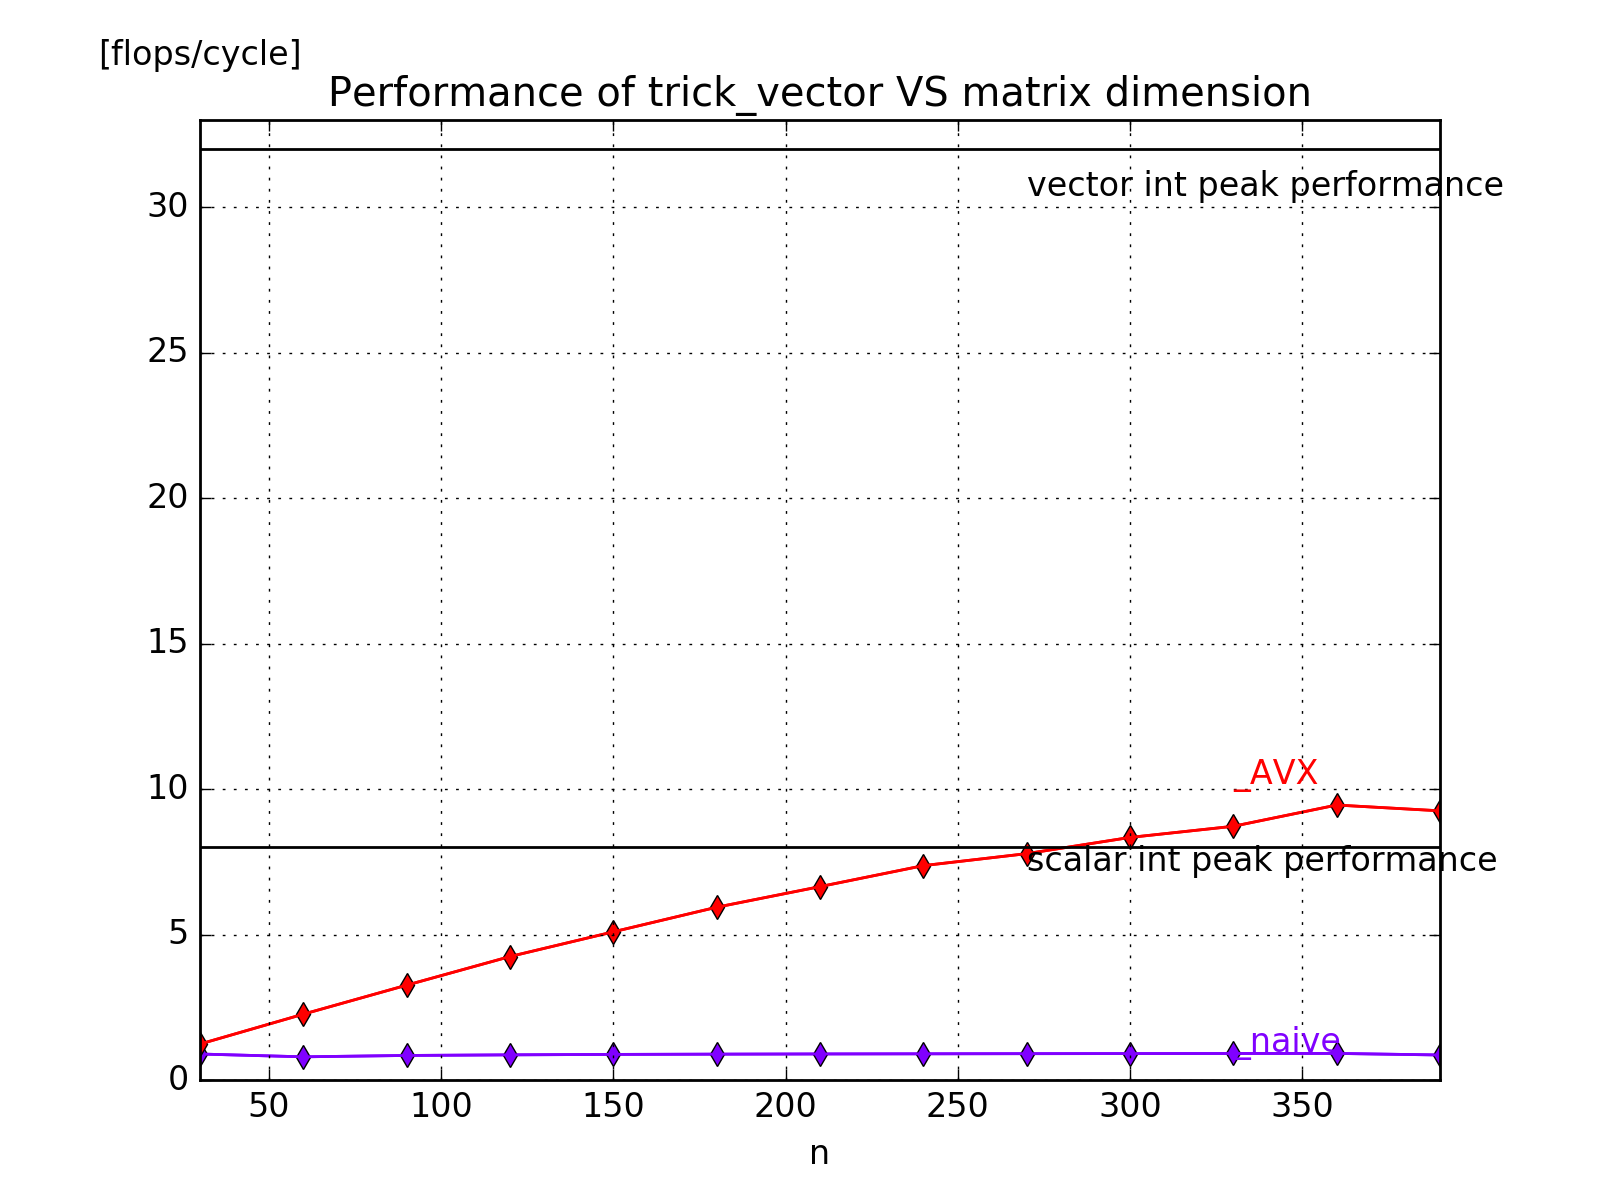
\includegraphics[width=0.5\textwidth]{Performance_trick_vector.eps}
\caption{Performance plot of the function \emph{trick\_vector}}
\label{figure:performance_trick_vector}
\end{figure}

\begin{figure}[h]
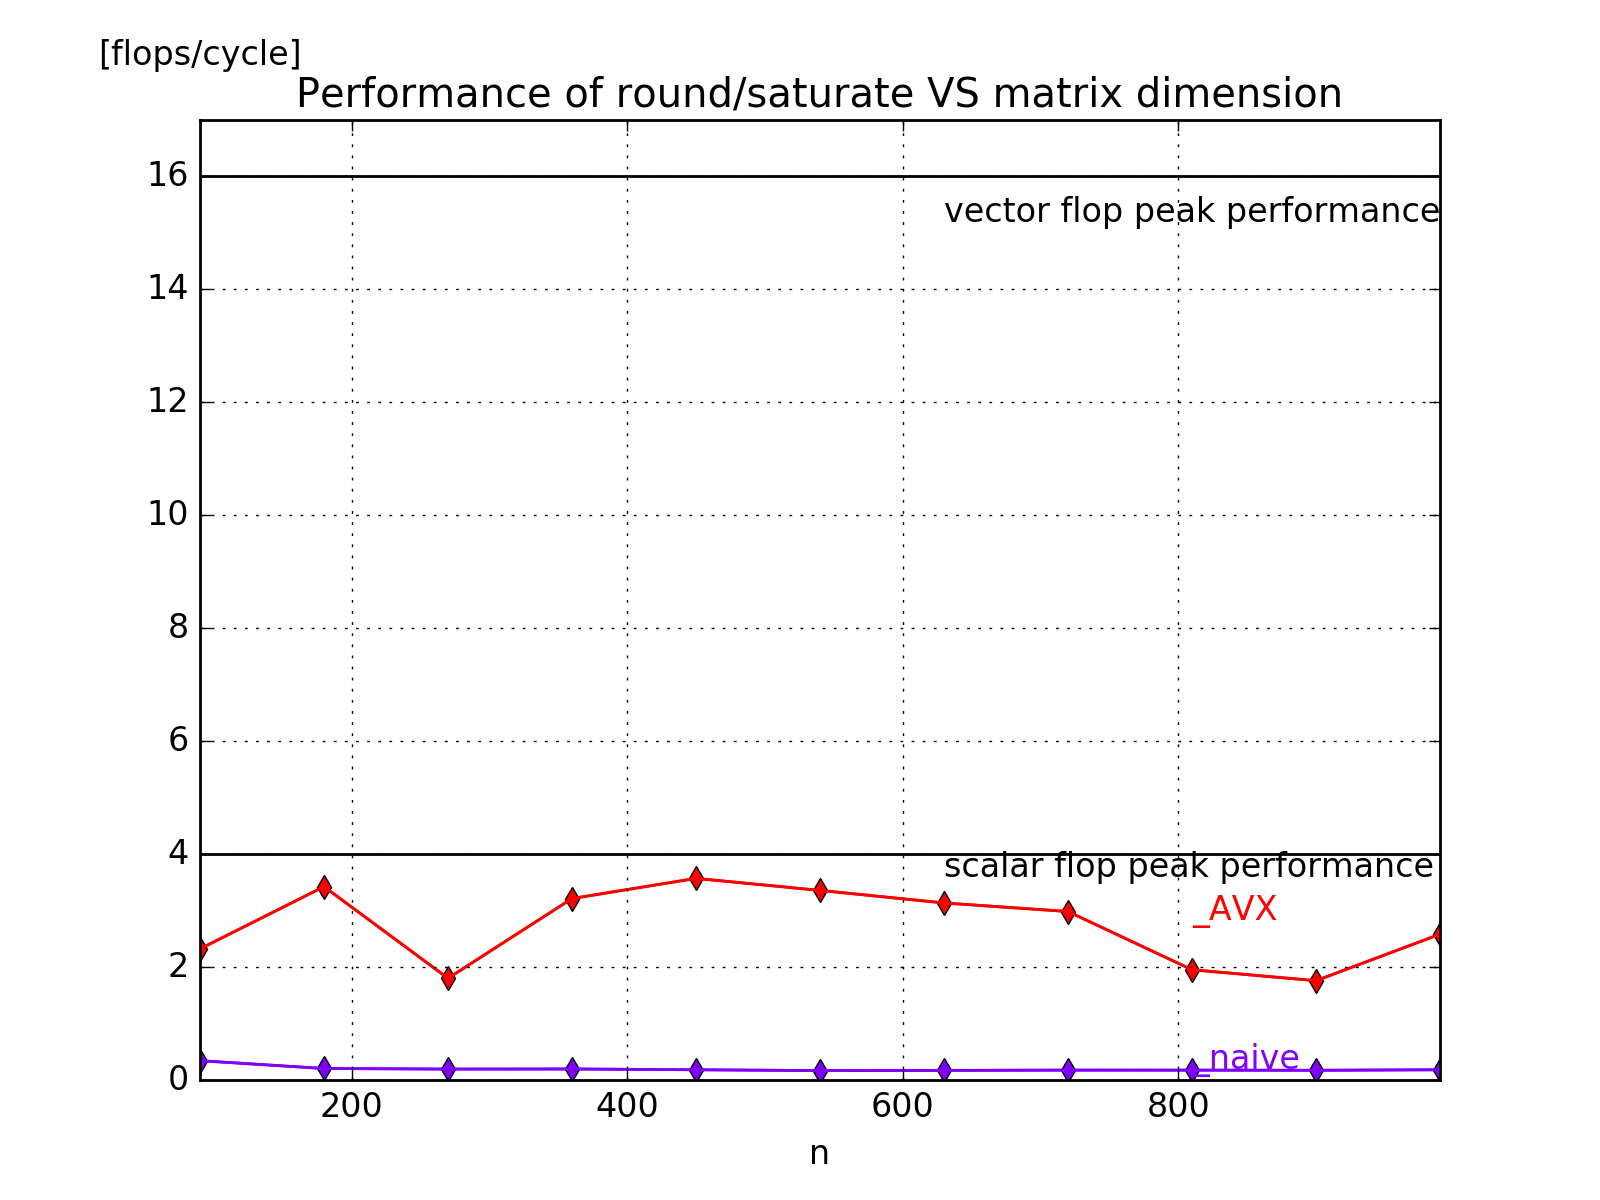
\includegraphics[width=0.5\textwidth]{Performance_round_saturation.eps}
\caption{Performance plot of the function \emph{round\_saturation}}
\label{figure:performance_round_saturation}
\end{figure}

The maximal gain in performance that the vectorization can allow for the functions \emph{trick\_vector} and \emph{add\_trick\_vector} is $16$X, that is the size of the accumulator vector for 16 bit integers. The measured performance gain are respectively  $9.8$X and $8.5$X.

\Cref{figure:performance_quantize} and \cref{figure:performance_round_saturation} show the performance plot for the functions \emph{quantize} and \emph{round\_saturation}. The measured performance gain are respectively $9.2$X and $14.2$X. 

In \cref{figure:cycles_qmm_comparison} we can see the runtime plot for the whole pipeline. The implementation \emph{trick\_blocking\_AVX} is obtained combining the \emph{QMM\_kernel\_blocking} with the vectorized implementation of all the other sub-functions. The overall speedup is $2.5$X.